\section{Validaci\'on}

El modelo propuesto para recuperar la ecuaci\'on de M\'arkus y H\'azi fue probado mediante la realizaci\'on de una serie de experimentos num\'ericos, destinados a evaluar la capacidad y precisi\'on para simular problemas de flujo multif\'asico con transferencia de calor y cambio de fase. En primer lugar, se obtuvieron soluciones num\'ericas para dos situaciones en las que es posible encontrar una soluci\'on anal\'itica: la estratificaci\'on de un fluido van der Waals en una cavidad con temperatura no uniforme, y la simulaci\'on de un frente de evaporaci\'on. Por otro lado, se simul\'o la generaci\'on de burbujas sobre una placa horizonal calefaccionada, tambi\'en conocido como ebullici\'on heterog\'enea, y se emple\'o este problema para discutir aspectos fundamentales de una simulaci\'on con lattice Boltzmann, como resoluci\'on de grilla y selecci\'on de condiciones de contorno.

\red{condiciones de contorno}
\red{ecuaci\'on de van der Waals}



\subsection{Estratificaci\'on de un fludo van der Waals}

La \eq{eq:vdw_column_red} permite describir la distribuci\'on unidimensional de densidad en un fluido van der Waals estratificado, de modo que se determina la variaci\'on de densidad en cada fase a partir de una \'unica interfase. sin embargo, a diferencia de la propuesta de Berberan-Santos \cite{berberan-santos_liquidvapor_2002}, en este caso es posible que la cavidad presente una distribuci\'onde temperatura no uniforme \cite{fogliatto_simulation_2019}. Esta flexibilidad adicional permite que este mismo problema pueda ser empleado para validar la \lbe{} propuesta. En particular, es sencillo ver que en un caso hidrost\'atico, la \eq{eq:markus_orig} puede expresarse en unidades reducidas como
\begin{equation}
	\dfrac{\partial}{\partial E_r} \left( \lambda \dfrac{\partial T_r}{\partial E_r} \right) = 0.
	\label{eq:markus_1d}
\end{equation}

Por lo tanto, para obtener una soluci\'on compatible con la \lbe{} dada por la \eq{eq:modelo_2d_full}, se completa el algoritmo descripto en la \se{sec:vdw_1d} con la incorporaci\'on de la resoluci\'on de la \eq{eq:markus_1d} usando el esquema de Patankar \cite{patankar_numerical_1980} con condiciones de temperatua fija en los extremos del dominio. De esta manera, actualizando la distribuci\'on de temperatura en el paso 4 y resolviendo de forma iterativa, es posible calcular una distribuci\'on de densidad en un dominio con una distribuci\'on de temperatura que depende del perfil de densidad final. 

Siguiendo el problema detallado en la \se{sec:vdw_1d}, se realizaron simulaciones sobre  una cavidad bidimensional con $H=300$, $L=3$ y condiciones de contorno peri\'odicas en la direcci\'on $x$. En este caso se consider\'o $E_r(H)=10^{-3}$ y una densidad inicial correspondiente al valor cr\'itico ($\rho_r = 1$) con una perturbaci\'on de $\pm 1 \%$.  Para el modelo isot\'ermico se consideraron los mismos factores de relajaci\'on y constates de simulaci\'on, con $M=1$, $G=-1$, $R=1$, $a=0.5$, $b=4$, $\tau_{\rho} = \tau_j=1$, $\tau_{e}^{-1}=\tau_{\zeta}^{-1}=\tau_{q}^{-1}=\tau_{\nu}^{-1}=1.1$, y $\sigma = 0.125$. Por otro lado, para la ecuaci\'on de energ\'ia se emplearon factores de relajaci\'on $q_i = 1$, $c_v = 4$, y par\'ametros libres de la distribuci\'on de equilibrio dados por $\alpha_1 = -1$ y $\alpha_2 = 1$. 

En una primera prueba num\'erica se fij\'o el valor de temperatura de la cara superior en $T_t = 0.99 T_c$, y se realizaron simulaciones para diferentes valores de temperatura en la cara inferior ($T_b$). Las \figs{fig:vdWColumnHT_rhor}{fig:vdWColumnHT_Tr} muestran las distribuciones de densidad y temperatura obtenidas para diferentes valores de $T_b$, donde se observa que, de forma similar a lo que ocurre con el problema isot\'ermico, la fase m\'as densa ocupa la parte inferior del dominio. Sin embargo, en este caso la distribuci\'on de temperatura final no es uniforme o fija, sino que presenta un perfil asociado a una ecuaci\'on de energ\'ia con difusividad t\'ermica constante. Esta restricci\'on determina que el perfil de $T$ presente una variaci\'on significativa en la zona de la fase de vapor, efecto que se acent\'ua con la disminuci\'on de la temperatura de la cara inferior.

La soluci\'n de este problema con lattice Boltzmann reproduce campos macrosc\'opicos con similares caracter\'isticas a los del modelo isot\'ermico, es decir, perfiles de densidad y temperatura similares a la soluci\'on anal\'itica en el seno del fluido, y con una interfase cuyo espesor disminuye con la temperatura. En este caso, la \lbe{} propuesta produce una distribuci\'on de temperatura continua a lo largo de la cavidad, mientras que el espesor no nulo de la interfase no afecta significativamente a la distribuci\'on de $T$ en la zona de la separaci\'on.

\begin{figure}[ht]
	\centering
	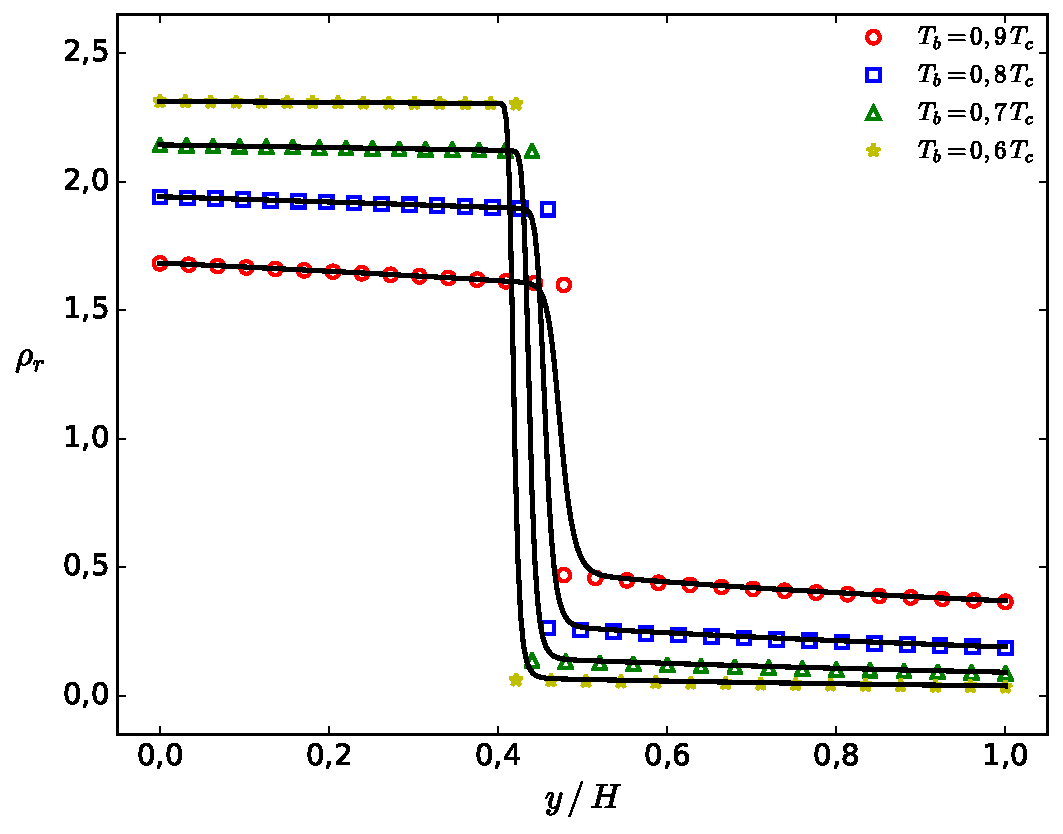
\includegraphics[width=0.75\textwidth]{vdWColumnHT_2D/CasoA/rhor_vdWcolumnHT}
	\caption{Distribuci\'on espacial de densidad en una cavidad con diferentes temperaturas en la cara inferior. Las l\'ineas continuas corresponden a simulaciones de lattice Boltzmann.}
	\label{fig:vdWColumnHT_rhor}
\end{figure}

\begin{figure}[ht]
	\centering
	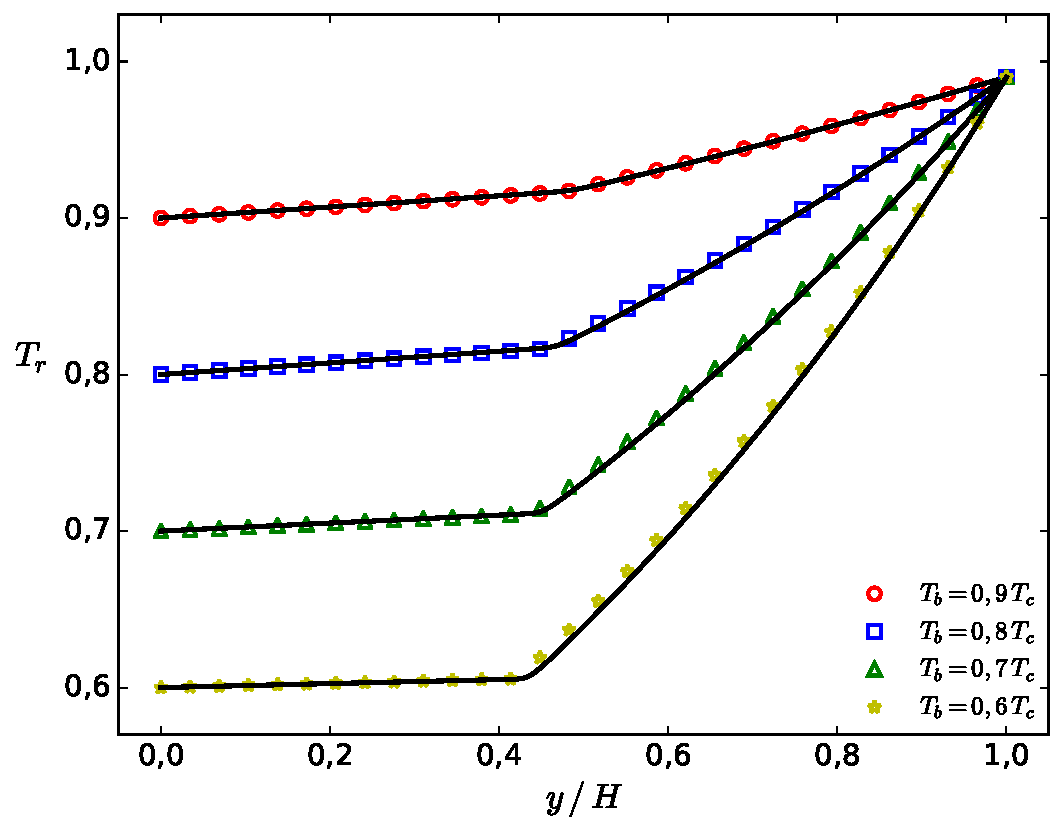
\includegraphics[width=0.75\textwidth]{vdWColumnHT_2D/CasoA/Tr_vdWcolumnHT}
	\caption{Distribuci\'on espacial de temperatura en una cavidad con diferentes temperaturas en la cara inferior. Las l\'ineas continuas corresponden a simulaciones de lattice Boltzmann.}
	\label{fig:vdWColumnHT_Tr}
\end{figure}

El problema de la cavidad constituye un excelente caso para evaluar los efectos de la resoluci\'on espacial en la reproducci\'on de la interfase. En la \fig{fig:vdWColumnHT_rhor_grilla} se muestran los perfiles de densidad reducida simulada con diferentes unidades de grilla en la direcci\'on vertical, usando $T_t = 0.99 \, T_c$ y $T_b = 0.8 \, T_c$. De forma similar a lo que ocurre con la simulaci\'on usando \'unicamente el modelo isot\'ermico, puede confirmarse que si se aplica una adimensionalizaci\'on apropiada (en variables reducidas), la concordancia entre la simulaci\'on y la soluci\'on anal\'itica mejora con el incremento de la resoluci\'on espacial. Es importante destacar que para este caso, el perfil de temperatura presenta un excelente acuerdo con la soluci\'on anal\'itica, como se muestra en la \fig{fig:vdWColumnHT_Tr}, de modo que no se observan cambios apreciables entre las diferentes resoluciones empleadas.

\begin{figure}[ht]
	\centering
	\includegraphics[width=0.75\textwidth]{vdWColumnHT_2D/CasoB/rhor_vdWcolumnHT_grilla}
	\caption{Distribuci\'on espacial de densidad en una cavidad con $T_b = 0.8 \, T_c$, $E_r(H)=10^{-3}$ y diferentes $H$. Las l\'ineas continuas corresponden a simulaciones de lattice Boltzmann.}
	\label{fig:vdWColumnHT_rhor_grilla}
\end{figure}

Como se observ\'o en el cap\'itulo anterior, las constantes de la ecuaci\'on de estado juegan un papel fundamental en la precisi\'on de la simulaci\'on para describir los perfiles de densidad y temperatura a trav\'es de la interfase. Las \figs{fig:vdWColumnHT_rhor_a_eos}{fig:vdWColumnHT_rhor_b_eos} muestran la distribuci\'on de densidad en una cavidad con $T_t = 0.99 \, T_c$ y $T_b = 0.8 \, T_c$, obtenidas con $b=4$ y variando $a$, y con $a=0.5$ pero cambiando $b$. Puede verse que en ambos casos, incrementando $a$ o reduciendo $b$, se reduce el espesor de la interfase en unidades de grilla mientras que se mantienen los perfiles de densidad reducidos en el seno de cada fase. Por otro lado, la disminuci\'on del par\'ametro $b$ aumenta la diferencia entre las densidades de l\'iquido y vapor, mientras que el incremento de $a$ y decremento de $b$ aumenta el gradiente del potencial de interacci\'on. Ambos efectos contribuyen a mejorar la capacidad del modelo \pp{} de reproducir adecuadamente la interfase, lo que induce a las tendencias mostradas en las \figs{fig:vdWColumnHT_rhor_a_eos}{fig:vdWColumnHT_rhor_b_eos}. La consecuencia fundamental radica en que los efectos sobre la soluci\'on adimensional son similares a los observados cuando se incrementa la resoluci\'on de grilla, aunque como ya se mencion\'o previamente, las mejoras de precisi\'on alcanzadas por este camino se encuentran limitadas por restricciones de estabilidad.

\begin{figure}[ht]
	\centering
	\includegraphics[width=0.75\textwidth]{vdWColumnHT_2D/CasoC/rhor_vdWcolumnHT_a_eos}
	\caption{Distribuci\'on espacial de densidad en una cavidad con $T_t = 0.99 \, T_c$ y $T_b = 0.8 \, T_c$. Las l\'ineas continuas corresponden a simulaciones de lattice Boltzmann con $b=4$ y distintos valores de $a$.}
	\label{fig:vdWColumnHT_rhor_a_eos}
\end{figure}

\begin{figure}[ht]
	\centering
	\includegraphics[width=0.75\textwidth]{vdWColumnHT_2D/CasoD/rhor_vdWcolumnHT_b_eos}
	\caption{Distribuci\'on espacial de densidad en una cavidad con $T_t = 0.99 \, T_c$ y $T_b = 0.8 \, T_c$. Las l\'ineas continuas corresponden a simulaciones de lattice Boltzmann con $a=0.5$ y distintos valores de $b$.}
	\label{fig:vdWColumnHT_rhor_b_eos}
\end{figure}
\FloatBarrier



\subsection{Frente de evaporaci\'on}

Otro caso de estudio relevante para validar modelos de lattice Boltzmann con cambio de fase consiste en la simulaci\'on de un frente de evaporaci\'on, tambi\'en conocido como flujo de Stefan unidimensional \cite{alexiades_mathematical_1993}. Como se muestra en la \fig{fig:Stefan_cavity}, el problema puede describirse como una cavidad unidimensional, con un extremo abierto, e inicialmente llena de l\'iquido a temperatura de saturaci\'on $T_s$. Si la temperatura del extremo cerrado ($T_w$) supera el valor de saturaci\'on, es decir $T_w > T_s$, comienza a producirse un cambio de fase en esta zona, y la evoluci\'on de la posici\'on de la interfase puede aproximarse anal\'iticamente. 

\begin{figure}[ht]
	\centering
	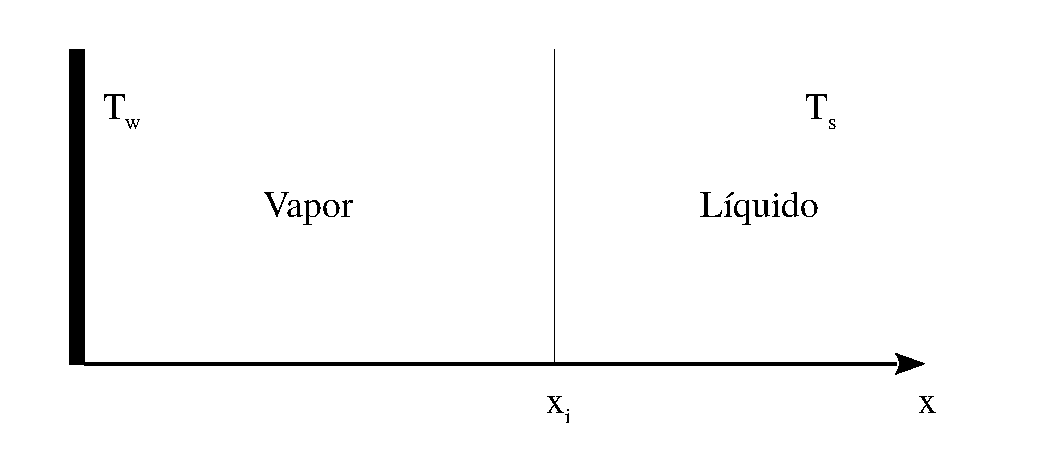
\includegraphics[width=0.75\textwidth]{Stefan/Stefan}
	\caption{Definici\'on del problema de flujo de Stefan}
	\label{fig:Stefan_cavity}
\end{figure}

El libro de Alex\'iades y Solomon \cite{alexiades_mathematical_1993} contiene una descripci\'on detallada sobre la obtenci\'on de soluciones anal\'iticas para diferentes problemas de cambio de fase, de modo que aqu\'i s\'olo se muestra un breve resumen del problema a evaluar. En el caso de inter\'es, la fase de vapor puede considerarse en reposo, de modo que la ecuaci\'on de energ\'ia en esta regi\'on se reduce a 
\begin{equation}
	\dfrac{\partial T}{\partial t} = \chi \dfrac{\partial^2 T}{\partial x^2}, \qquad 0 < x < x_i(t),
\end{equation}
donde $x_i(t)$ corresponde a la posici\'on de la interfase que cambia en el tiempo. Si se imponen condiciones de contorno de Dirichlet para la regi\'on de vapor, es decir
\begin{subequations}
	\begin{equation}
		T(x=0,t) = T_w
	\end{equation}
	\begin{equation}
		T(x=x_i(t),t) = T_s,
	\end{equation}	
\end{subequations}
entonces el problema es resoluble si se considera una condici\'on de salto de energ\'ia sobre la interfase:
\begin{equation}
	\rho_g u_i h_{fg} = -\lambda_g \left.\dfrac{\partial T}{\partial x} \right|_{x=x_i(t)},
\end{equation}
donde $u_i=dx_i/dt$, $h_{fg}$ es el calor latente y $\lambda_g$ la conductividad t\'ermica de la fase de vapor. Con estas aproximaciones, la posici\'on de la interfase en funci\'on del tiempo puede estimarse como:
\begin{equation}
	x_i(t)=2\beta \sqrt{\chi_lt},
	\label{eq:stefan_int}
\end{equation},
donde $\chi_l$ corresponde a la difusividad t\'ermica de la fase l\'iquida y $\beta$ satisface la siguiente ecuaci\'on trascendental:
\begin{equation}
	\beta \mbox{e}^{\beta^2}\mbox{erf}(\beta)=\dfrac{c_{pg}(T_w-T_s)}{h_{fg}\sqrt{\pi}} = \dfrac{St}{\sqrt{\pi}}.
	\label{eq:stefan_beta}
\end{equation}

En la \eq{eq:stefan_beta} $c_{pg}$ es el calor espec\'ifico a presi\'on constante de la fase de vapor y $St$ se conoce como el n\'umero de Stefan. 

La descripci\'on de la din\'amica del frente de vapor asume que la temperatura de la interfase y de toda la regi\'on de fluido es igual a $T_s$. Por otro lado, la fase de vapor se encuentra en reposo, y el movimiento de la interfase desplaza la columna de l\'quido con velocidad uniforme (pero no constante en el tiempo) hacia el extremo abierto del dominio. Estas hip\'otesis sobre la soluci\'on anal\'itica imponen restricciones al momento de emplear este problema como caso de prueba de un modelo de lattice Boltzmann, aunque ya ha sido utilizado satisfactoriamente por Safari y colaboradores \cite{safari_consistent_2014} para validar un modelo t\'ermico de la familia phase-field. Sin embargo, a diferencia de un modelo phase-field, en un modelo \pp{} no es posible fijar la temperatura de la interfase, por lo que es necesario recurrir a una condici\'on de simulaci\'on que permita sobreponer parcialmente esta restricci\'on. En particular, si se recupera una ecuaci\'on de energ\'ia con $\chi$ constante en cada fase, entonces la construcci\'on de un caso computacional donde $\rho_l \gg \rho_g$ produce $\lambda_l \gg \lambda_g$, y por lo tanto la temperatura sobre la interfase se asemeja a la del extremo del dominio computacional $T_s$.

La evoluci\'on de un frente de evaporaci\'on se simul\'o con lattice Boltzmann usando un dominio de $L=600$ unidades de grilla en la direcci\'on $x$ y s\'olo $H=3$ en la direcci\'on $y$, ya que no se observaron diferencias significativas en simulaciones realizadas sobre grillas con m\'as elementos en la direcci\'on peri\'odica. La cantidad elegida de nodos en la direcci\'on principal reduce efectos de la condici\'on de contorno en el extremo abierto sobre el interior del dominio. En todos los casos se impusieron condiciones de temperatura fija en los extremos del dominio con $T(L) = 0.8 \, T_c$, de no deslizamiento en $x=0$, y de flujo saliente (\emph{outflow}) para densidad y velocidad en $x=L$ \cite{lou_evaluation_2013}. En esta \'ultima condici\'on, los valores de $\rho$ y $\bm{u}$ sobre los nodos de la frontera se obtienen a partir de una interpolaci\'on considerando nodos del interior y una velocidad de advecci\'on. De esta forma, las componentes de $\bm{f}$ son actualizadas despu\'es del paso de \emph{streaming} para satisfacer los momentos macrosc\'opicos extrapolados.

Las constantes de simulaci\'on empleadas en las \lbe{} hidrodin\'amica y de energ\'ia se encuentran en las \tabs{}{} respectivamente \red{poner tablas}. Inicialmente, el dominio se encuentra a temperatura uniforme $T_r = 0.8$, y la distribuci\'on de densidad es uniforme e igual a la de coexistencia de la fase l\'iquida a $T_r = 0.8$. Si se deja evolucionar un sistema con esta configuraci\'on, inicialmente se produce una zona de vapor en $x=0$ sin necesidad de incluir un disparador adicional, como puede ser una peque\~na regi\'on de vapor, y la posici\'on de la interfase de desplaza hasta alcanzar $x=L$. La \fig{fig:Stefan_m1_1} muestra la posici\'on de la interfase calculada usando diferentes valores de $T_w$, lo cual se refleja en distintos n\'umeros de Stefan. 

\begin{figure}[ht]
	\centering
	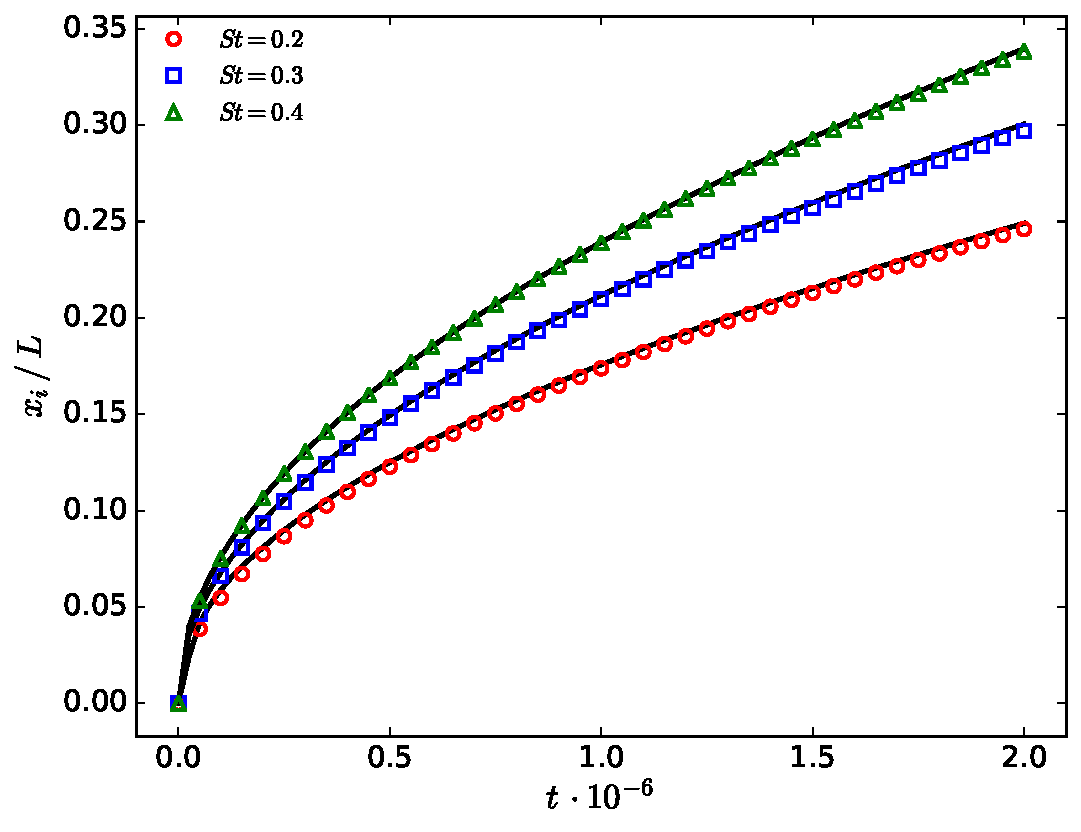
\includegraphics[width=0.75\textwidth]{Stefan/2D/CasoA/Stefan_m1_1}
	\caption{Posici\'on del frente de evaporaci\'on para diferentes n\'umeros de Stefan, con $\alpha_1 = -1$, $\alpha_2=1$ y $q_{\chi} = 1.8$. Las l\'ineas s\'olidas corresponden a las simulaciones con lattice Boltzmann}
	\label{fig:Stefan_m1_1}
\end{figure}

Las soluciones anal\'iticas fueron estimadas usando $h_{fg}=h_g-h_l$, donde la entalp\'ia de cada fase puede determinarse anal\'iticamente a partir de la ecuaci\'on de estado de van der Waals \cite{markus_simulation_2011}:
\begin{equation}
	h = \left( \dfrac{3}{2} \dfrac{1}{1-b\rho} \right)RT - 2b\rho.
\end{equation}

La evoluci\'on de la interfase mostrada en la \fig{Stefan_m1_1} indica que el modelo propuesto puede reproducir satisfactoriamente la estimaci\'on dada por las \eqs{eq:stefan_int}{eq:stefan_beta}, lo que implica que la transferencia de masa a trav\'es de las interfase puede ser recuperada correctamente cuando el cambio de fase est\'a governado por una ecuaci\'on de estado, sin necesidad de reconstruir la interfase o de efectuar aproximaciones adicionales.

En este punto, y tomando como base los resultados del frente de evaporaci\'on, es posible mostrar que la \lbe{} propuesta para recuperar la ecuaci\'on de energ\'ia tiene la capacidad de reducir posibles restricciones de estabilidad asociadas al uso de valores grandes de $q_{\chi}$, ya que como se aprecia en la \eq{eq:modelo_2d_chi}, la difusividad t\'ermica tambi\'en puede ser ajustada mediante $\alpha_1$ y $\alpha_2$. Para ilustrar esta caracter\'istica, se realizaron simulaciones del frente de evaporaci\'on usando $\alpha_1=-2$, $\alpha_2=2$ y $q_{\chi}=1.7143$, lo que formalmente reproduce la misma difusividad t\'ermica que $\alpha_1=-1$, $\alpha_2=1$ y $q_{\chi}=1.8$, y por lo tanto, el mismo resultado f\'isico. Como se aprecia en la \fig{fig:Stefan_m2_2}, la evoluci\'on del frente de evaporaci\'on no se distingue de aquella obtenida mediante otro conjunto de par\'ametros (\fig{fig:Stefan_m1_1}), lo que indica que la difusividad t\'ermica recuperada es la misma en ambos casos. Esta capacidad de usar diferentes factores de relajaci\'on para lograr un mismo valor de $\chi$ puede ser utilizada para compensar simulaciones num\'ericamente inestables.

\begin{figure}[ht]
	\centering
	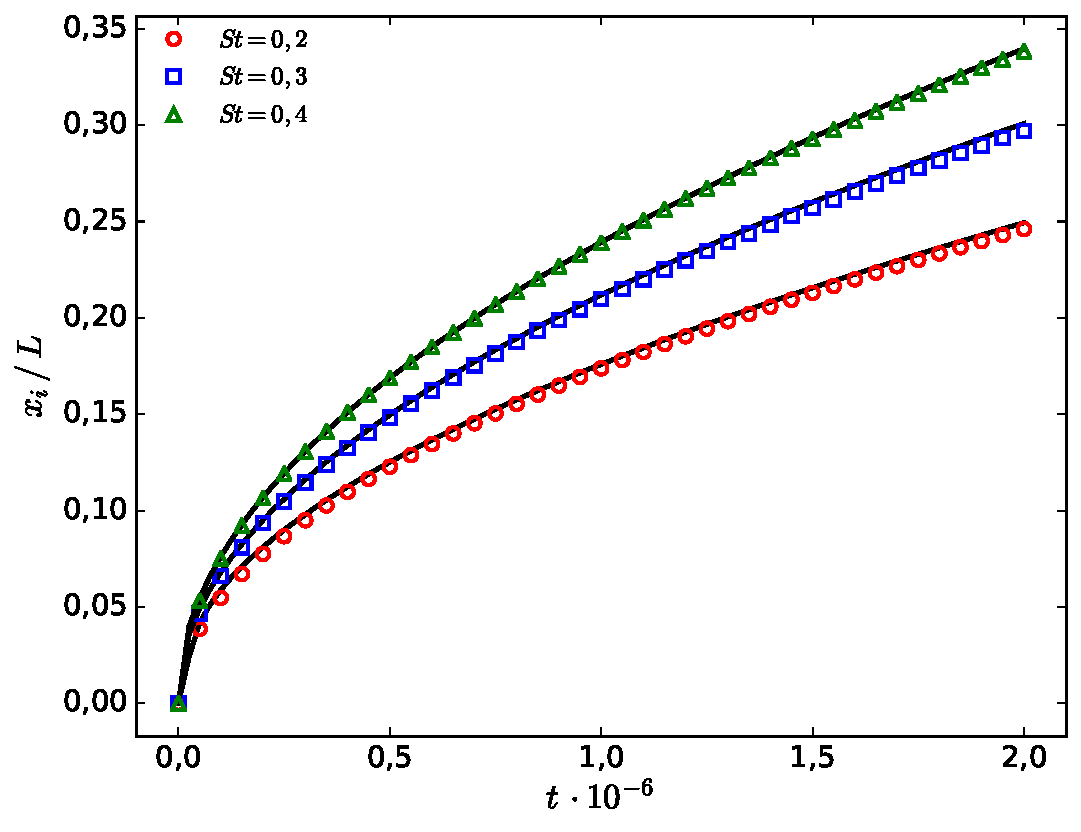
\includegraphics[width=0.75\textwidth]{Stefan/2D/CasoB/Stefan_m2_2}
	\caption{Posici\'on del frente de evaporaci\'on para diferentes n\'umeros de Stefan, con $\alpha_1 = -2$, $\alpha_2=2$ y $q_{\chi} = 1.7143$. Las l\'ineas s\'olidas corresponden a las simulaciones con lattice Boltzmann}
	\label{fig:Stefan_m2_2}
\end{figure}










\subsection{Ebullici\'on heterog\'enea}